% ML Systems Stack Diagram Prototype
% This is a standalone test file - compile with pdflatex to preview

\documentclass[border=10pt]{standalone}
\usepackage{tikz}
\usetikzlibrary{positioning}
\usepackage{xcolor}

% Define colors
\definecolor{crimson}{HTML}{A51C30}
\definecolor{lightgray}{HTML}{E8E8E8}
\definecolor{medgray}{HTML}{B0B0B0}

\begin{document}

% =============================================================================
% VERSION 1: Simple clean stack (like Harris & Harris)
% =============================================================================
% Example: DL Primer chapter - highlights Accelerators, Runtimes, Frameworks

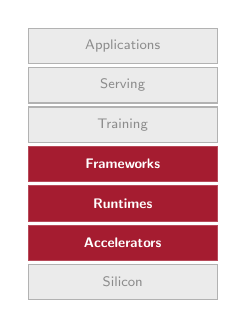
\begin{tikzpicture}[
    layer/.style={
        draw=black!30,
        minimum width=2.4cm,
        minimum height=0.45cm,
        font=\sffamily\tiny,
        align=center,
    },
    highlighted/.style={
        layer,
        fill=crimson,
        text=white,
        draw=crimson!80,
        font=\sffamily\tiny\bfseries,
    },
    unhighlighted/.style={
        layer,
        fill=black!8,
        text=black!45,
    },
]

\node[unhighlighted] (L1) at (0, 0) {Silicon};
\node[highlighted] (L2) at (0, 0.5) {Accelerators};
\node[highlighted] (L3) at (0, 1.0) {Runtimes};
\node[highlighted] (L4) at (0, 1.5) {Frameworks};
\node[unhighlighted] (L5) at (0, 2.0) {Training};
\node[unhighlighted] (L6) at (0, 2.5) {Serving};
\node[unhighlighted] (L7) at (0, 3.0) {Applications};

\end{tikzpicture}

\hspace{1cm}

% =============================================================================
% VERSION 2: With gradient for partial relevance
% =============================================================================
% Example: DL Primer - primary focus on Frameworks/Runtimes, touches Accelerators/Training

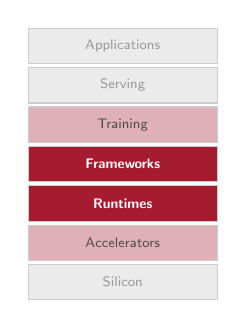
\begin{tikzpicture}[
    layer/.style={
        draw=black!20,
        minimum width=2.4cm,
        minimum height=0.45cm,
        font=\sffamily\tiny,
        align=center,
    },
]

% Gradient: full=100%, partial=35%, none=8%
\node[layer, fill=black!8, text=black!40] (L1) at (0, 0) {Silicon};
\node[layer, fill=crimson!35, text=black!70] (L2) at (0, 0.5) {Accelerators};
\node[layer, fill=crimson, text=white, font=\sffamily\tiny\bfseries] (L3) at (0, 1.0) {Runtimes};
\node[layer, fill=crimson, text=white, font=\sffamily\tiny\bfseries] (L4) at (0, 1.5) {Frameworks};
\node[layer, fill=crimson!35, text=black!70] (L5) at (0, 2.0) {Training};
\node[layer, fill=black!8, text=black!40] (L6) at (0, 2.5) {Serving};
\node[layer, fill=black!8, text=black!40] (L7) at (0, 3.0) {Applications};

\end{tikzpicture}

\hspace{1cm}

% =============================================================================
% VERSION 3: HW Acceleration chapter
% =============================================================================

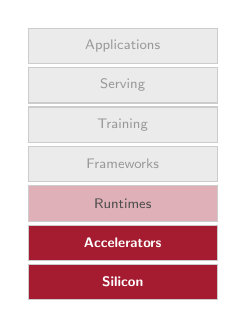
\begin{tikzpicture}[
    layer/.style={
        draw=black!20,
        minimum width=2.4cm,
        minimum height=0.45cm,
        font=\sffamily\tiny,
        align=center,
    },
]

\node[layer, fill=crimson, text=white, font=\sffamily\tiny\bfseries] (L1) at (0, 0) {Silicon};
\node[layer, fill=crimson, text=white, font=\sffamily\tiny\bfseries] (L2) at (0, 0.5) {Accelerators};
\node[layer, fill=crimson!35, text=black!70] (L3) at (0, 1.0) {Runtimes};
\node[layer, fill=black!8, text=black!40] (L4) at (0, 1.5) {Frameworks};
\node[layer, fill=black!8, text=black!40] (L5) at (0, 2.0) {Training};
\node[layer, fill=black!8, text=black!40] (L6) at (0, 2.5) {Serving};
\node[layer, fill=black!8, text=black!40] (L7) at (0, 3.0) {Applications};

\end{tikzpicture}

\hspace{1cm}

% =============================================================================
% VERSION 4: Serving chapter
% =============================================================================

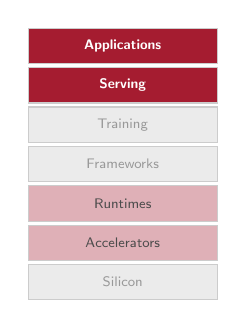
\begin{tikzpicture}[
    layer/.style={
        draw=black!20,
        minimum width=2.4cm,
        minimum height=0.45cm,
        font=\sffamily\tiny,
        align=center,
    },
]

\node[layer, fill=black!8, text=black!40] (L1) at (0, 0) {Silicon};
\node[layer, fill=crimson!35, text=black!70] (L2) at (0, 0.5) {Accelerators};
\node[layer, fill=crimson!35, text=black!70] (L3) at (0, 1.0) {Runtimes};
\node[layer, fill=black!8, text=black!40] (L4) at (0, 1.5) {Frameworks};
\node[layer, fill=black!8, text=black!40] (L5) at (0, 2.0) {Training};
\node[layer, fill=crimson, text=white, font=\sffamily\tiny\bfseries] (L6) at (0, 2.5) {Serving};
\node[layer, fill=crimson, text=white, font=\sffamily\tiny\bfseries] (L7) at (0, 3.0) {Applications};

\end{tikzpicture}

\hspace{1cm}

% =============================================================================
% VERSION 5: Introduction chapter (all layers highlighted)
% =============================================================================

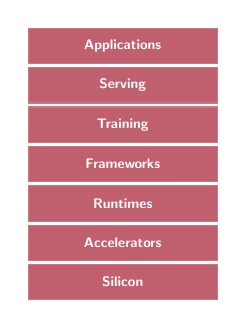
\begin{tikzpicture}[
    layer/.style={
        draw=crimson!60,
        minimum width=2.4cm,
        minimum height=0.45cm,
        font=\sffamily\tiny\bfseries,
        align=center,
        fill=crimson!70,
        text=white,
    },
]

\node[layer] (L1) at (0, 0) {Silicon};
\node[layer] (L2) at (0, 0.5) {Accelerators};
\node[layer] (L3) at (0, 1.0) {Runtimes};
\node[layer] (L4) at (0, 1.5) {Frameworks};
\node[layer] (L5) at (0, 2.0) {Training};
\node[layer] (L6) at (0, 2.5) {Serving};
\node[layer] (L7) at (0, 3.0) {Applications};

\end{tikzpicture}

\end{document}
